% !TEX program = xelatex
% Шаблон научной статьи НИТУ «МИСиС»
% Заполните блоки ниже и скомпилируйте: xelatex article.tex

\documentclass{misisarticle}
\usepackage{pgfplots}
\pgfplotsset{compat=1.17}
\raggedbottom

% --- Классификационные коды (оставьте пустым {}, если не требуются) ---
% ГРНТИ: Распознавание образов. Обработка изображений
\grnti{28.23.15}
% ASJC: Signal Processing
\asjc{1711}
% OECD: Computer and information sciences
\oecd{1.2}

% --- Название ---
\title{Обнаружение и оценка параметров движения БПЛА по данным наземного LiDAR}

% --- Авторы: \misisauthor{ФИО}{аффилиация}{город, страна}{email} ---
% TODO: уточнить аффилиации, города и email авторов; пока оставлены данные шаблона.
\misisauthor{Н.~О.~Зонтов\par А.~А.~Муромцев}{кафедра инженерной кибернетики НИТУ «МИСиС»}{Москва, Россия}{student@edu.misis.ru}
\misisauthor{М.~Р.~Вишневский}{кафедра инженерной кибернетики НИТУ «МИСиС»}{Москва, Россия}{supervisor@misis.ru}

% --- Аннотация и ключевые слова ---
\abstract{%
  Работа посвящена задаче автоматического обнаружения беспилотного летательного аппарата и оценки параметров его движения по данным наземного LiDAR. В качестве сенсора используется LiDAR Livox Horizon, формирующий трехмерные облака точек с non-repetitive паттерном сканирования. Предлагается алгоритм последовательной обработки облака точек, включающий предварительную фильтрацию данных, выделение объектов, идентификацию БПЛА и отслеживание его положения во времени. На основе последовательности обнаруженных координат строится траектория полета и оценивается скорость движения БПЛА. Для проверки работоспособности алгоритма будут самостоятельно сформированы датасеты с реальными полетами БПЛА на различных расстояниях и траекториях. Эффективность разработанного подхода будет оцениваться по точности обнаружения, точности восстановления траектории и оценке скорости движения БПЛА.
}

\keywords{%
  БПЛА, LiDAR, облако точек, обнаружение объектов, трекинг оценка скорости
}

\begin{document}

\maketitle

% ============================================================
\section{Введение}

При испытаниях беспилотного летательного аппарата (БПЛА) наземные измерения позволяют восстановить траекторию полёта независимо от бортовой телеметрии. Для этого необходимо определять положение аппарата в единой системе координат и связывать измерения, полученные в разные моменты времени. Задачи обнаружения и сопровождения БПЛА по трёхмерным облакам точек рассматриваются в работах~\cite{ref2,ref6}. В настоящей работе источником измерений служит неподвижный наземный лидар Livox Horizon.

В полевых записях значительная часть отражений приходится на поверхность земли, тогда как малоразмерный БПЛА представлен лишь небольшим скоплением точек. Число отражений от аппарата зависит от его дальности и положения в поле зрения. При неповторяющейся развёртке Livox Horizon последовательные сканы дополняют друг друга. Накопление сканов позволяет получить больше отражений от цели, однако за время накопления аппарат успевает сместиться. В результате точки в объединённом облаке могут соответствовать разным положениям БПЛА, что затрудняет оценку его мгновенных координат.

Цель работы~--- обнаружить БПЛА по данным наземного лидара и оценить по последовательности его положений траекторию и скорость полёта. В разработанном программном комплексе на базе ROS Noetic измерения нескольких сканов объединяются и обрабатываются воксельным фильтром. Затем методом RANSAC оценивается плоскость земли, а оставшиеся после её отделения точки группируются алгоритмом DBSCAN. Полученные группы служат кандидатами для обнаружения аппарата. Следующий этап исследования предусматривает выбор группы, соответствующей БПЛА, и сопоставление её положений во времени. На записях реальных полётов при разных дальностях и траекториях планируется оценить точность обнаружения, восстановления траектории и определения скорости.

% ============================================================
\section{Анализ работ}

В задачах оптического наблюдения качество обнаружения БПЛА обычно оценивают по тому, насколько точно детектор выделяет аппарат на изображении. Матяш~\cite{ref3} сравнил YOLOv8, ResNet50 и VGG-16 на фотографиях винтовых БПЛА. На использованной выборке YOLOv8 показала лучшие значения точности и полноты, однако автор отмечает трудности при малом размере изображения цели и частичном перекрытии аппарата. Бахвалов и Старцев~\cite{ref4} рассматривали также распознавание типа аппарата и размечали на изображениях два класса БПЛА --- самолётного и вертолётного типов. Для оценки движения в метрах одной ограничивающей рамки на снимке недостаточно. Требуется дополнительная информация о дальности до цели, которую наземный лидар измеряет непосредственно.

Для лидарного наблюдения существенны как число отражений от аппарата, так и возможность сопоставить их в соседних сканах. Abir и соавт.~\cite{ref2} исследовали влияние материала корпуса и условий видимости на дальность обнаружения. В полевых экспериментах с Livox Mid-40 авторы продемонстрировали сопровождение БПЛА на расстояниях до 80~м при съёмке в разное время суток. Эта дальность характеризует условия их эксперимента. Для Livox Horizon представляет интерес зависимость качества сопровождения от дальности при выбранном интервале накопления сканов. Другое решение задачи разреженности предложили Вишневский и Фёдоров~\cite{ref5}. В их системе дополнительный поток измерений формирует зеркало, а автоматическая калибровка позволяет совместить отражённые лучи с прямыми в общей системе координат. Такой способ повышает плотность измерений в выбранной области обзора механического лидара. При накоплении сканов Horizon источником дополнительных точек служат последовательные наблюдения, поэтому на форму облака влияет перемещение цели за время накопления.

Wang и соавт.~\cite{ref6} разделили обнаружение и сопровождение на два этапа. В облаке точек Livox Mid-40 они выделяли объекты методом евклидовой кластеризации, после чего сопровождали выбранную цель фильтром частиц. В системе Lucid история движения нужна также для распознавания объекта. Kim и соавт.~\cite{ref1} выделяют подвижные объекты с помощью пространственно-временного вычитания фона и используют траекторию для различения БПЛА и других движущихся целей. Это различие существенно для нашей задачи. Пространственно обособленная группа точек даёт кандидата для сопровождения, а отнесение группы к БПЛА требует дополнительных признаков.

При оценке метода на данных Livox Horizon важно различать две характеристики. Первая показывает, как часто удаётся выделить кластер БПЛА на заданной дальности. Вторая определяет, с какой погрешностью по положениям этого кластера в последовательных наблюдениях восстанавливаются траектория и скорость полёта.

\section{Наборы данных}

Для исследования используется запись наземного лидара Livox Horizon из набора \texttt{Drone\_livox}. За 153{,}24~с в канале \texttt{/livox/lidar} зарегистрировано 15\,325 облаков точек с частотой около 100~Гц. Для каждого измерения сохраняются координаты в системе лидара, интенсивность отражения, служебная метка и номер линии сканирования. Запись также содержит данные инерциального модуля в канале \texttt{/livox/imu}.

На рис.~\ref{fig:livox-frames} показаны два отдельных скана через 2 и 75~с после начала записи лидарных данных. В каждом кадре по 2400 записей. После исключения точек с координатами $(0,0,0)$ в первом скане остаётся 162 точки, во втором~--- 937. Примеры сохранены в CSV со всеми исходными полями точек. На графике цвет обозначает момент наблюдения.

\noindent\begin{minipage}{\columnwidth}
  \centering
  \begin{tikzpicture}
    \begin{axis}[width=\columnwidth,height=0.76\columnwidth,
      xlabel={$x$, м},ylabel={$y$, м},xmin=0,xmax=66,ymin=-33,ymax=35,
      tick label style={font=\footnotesize},legend style={font=\footnotesize},
      legend pos=north west,only marks,mark size=0.65pt,
      restrict x to domain=0.0001:66,filter discard warning=false]
      \addplot[mark=*,blue!55] table[x=x,y=y,col sep=comma]{data/livox_114302.csv};
      \addlegendentry{75 с}
      \addplot[mark=triangle*,red!75!black] table[x=x,y=y,col sep=comma]{data/livox_107002.csv};
      \addlegendentry{2 с}
    \end{axis}
  \end{tikzpicture}
  \captionof{figure}{Проекции двух сканов Livox Horizon на плоскость $xy$ в системе координат лидара.}
  \label{fig:livox-frames}
\end{minipage}\par

\section{Основная часть}

\subsection{Накопление сканов}

Обработка начинается с последовательности облаков точек, поступающих от неподвижного Livox Horizon. Из каждого сообщения извлекаются координаты $(x,y,z)$ в системе лидара. Объединяются 50 последовательных сканов, после чего буфер очищается. При частоте 100~Гц новое накопленное облако формируется примерно раз в 0{,}5~с. За это время лучи регистрируют отражения с разных участков поверхности. Для движущейся цели длительность окна ограничивает временное разрешение наблюдений.

\subsection{Воксельная фильтрация}

Чтобы уменьшить число точек перед поиском плоскости земли, накопленное облако разбивается на кубические ячейки. В базовой конфигурации ребро ячейки равно 0{,}05~м. Каждая занятая ячейка $V$ представляется одной точкой с координатами
\begin{equation}
  \bar{\mathbf p}_V = \frac{1}{n_V}
  \sum_{\mathbf p_i \in V} \mathbf p_i ,
\end{equation}
где $n_V$~--- число исходных точек в ячейке. В результате многократные отражения от одного участка земли дают при оценке плоскости один голос на занятую ячейку. Размер ячейки особенно важен для малой цели, поскольку при слишком крупной сетке близкие отражения от корпуса объединяются.

\subsection{Выделение поверхности земли}

Модель земли оценивается по первым четырём вокселизированным облакам. Метод RANSAC строит плоскости по тройкам точек и ищет модель с наибольшим числом согласованных измерений. Для плоскости с единичной нормалью $\mathbf n=(a,b,c)$ и смещением $d$ расстояние от точки $\mathbf p_i$ до плоскости равно
\begin{equation}
  r_i = \left|\mathbf n^\mathsf{T}\mathbf p_i+d\right|.
\end{equation}
Точка относится к земле при $r_i<\tau$. По умолчанию $\tau=0{,}1$~м. Условие $|c|>0{,}8$ ограничивает наклон допустимой плоскости относительно горизонтали. Если доминирующая плоскость слишком крутая, её точки исключаются из поиска и при достаточном числе оставшихся точек поиск повторяется. Для принятия модели требуется не менее 500 согласованных точек и не менее 5\% исходного набора для инициализации.

При неподвижной установке лидара принятую модель можно использовать для последующих облаков. На рис.~\ref{fig:ground-result} показан пример сегментации полевой записи. Над поверхностью земли видно компактное скопление точек, которое поступает на следующий этап вместе с другими отражениями вне плоскости.

\noindent\begin{minipage}{\columnwidth}
  \centering
  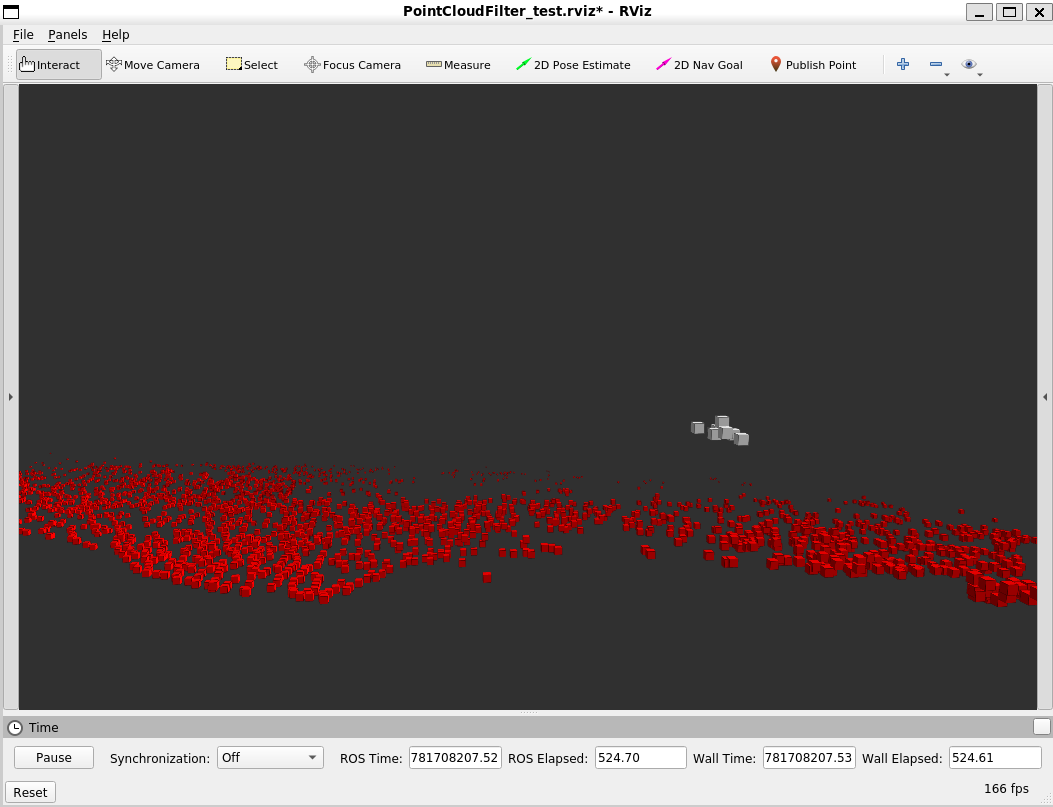
\includegraphics[width=\linewidth]{figures/ground-segmentation.png}
  \captionof{figure}{Результат сегментации в RViz. Красным показаны точки поверхности земли, светлым цветом~--- точки вне плоскости.}
  \label{fig:ground-result}
\end{minipage}\par

\subsection{Кластеризация точек объектов}

К оставшимся точкам применяется алгоритм DBSCAN. Для каждой точки $\mathbf p_i$ рассматривается окрестность
\begin{equation}
  N_\varepsilon(\mathbf p_i)=
  \{\mathbf p_j:\|\mathbf p_j-\mathbf p_i\|_2\leq\varepsilon\}.
\end{equation}
В базовой конфигурации $\varepsilon=0{,}15$~м. Точка считается ядром кластера, если в её окрестности находится не менее 30 точек, включая её саму. Соседние ядра объединяются в кластер, к которому присоединяются и граничные точки. В RViz каждому кластеру назначается цвет, а шумовые точки отображаются серым. Полученные метки описывают отдельное облако. Для восстановления траектории БПЛА требуется выбрать соответствующий ему кластер и сопоставить его с наблюдениями в последующие моменты времени.
% Список литературы — как в example/example.tex
\begin{thebibliography}{99}

\bibitem{ref1} Kim D., Paek J., Bahk S. Lucid: LiDAR-Based UAV Classification and Detection for Airspace Surveillance // Proceedings of the 2026 IEEE 46th International Conference on Distributed Computing Systems (ICDCS). --- 2026. --- P.~949--959. --- DOI: \href{https://doi.org/10.1109/2575-8411.2026.00095}{\nolinkurl{10.1109/2575-8411.2026.00095}}. --- URL: \url{https://ieeexplore.ieee.org/document/11619102} (дата обращения: 15.10.2026).

\bibitem{ref2} Abir T.~A., Kuantama E., Han R., Dawes J., Mildren R., Nguyen P. Towards Robust LiDAR-Based 3D Detection and Tracking of UAVs // DroNet IX: Proceedings of the 9th ACM Workshop on Micro Aerial Vehicle Networks, Systems, and Applications. --- New York : Association for Computing Machinery, 2023. --- P.~1--7. --- DOI: \href{https://doi.org/10.1145/3597060.3597236}{\nolinkurl{10.1145/3597060.3597236}}. --- URL: \url{https://dl.acm.org/doi/10.1145/3597060.3597236} (дата обращения: 15.10.2026).

\bibitem{ref3} Матяш Д.~С. Детекция беспилотных летательных аппаратов на фотографиях с использованием методов компьютерного зрения // Труды конференции. --- 2024. --- С.~92--99. --- URL: \url{https://elibrary.ru/item.asp?id=82411639&pff=1}.

\bibitem{ref4} Бахвалов И.~М., Старцев С.~В. Распознавание БПЛА различных классов средствами компьютерного зрения // Труды конференции. --- 2024. --- С.~34--40. --- URL: \url{https://elibrary.ru/item.asp?id=72973865&pff=1}.

\bibitem{ref5} Вишневский М.~Р., Фёдоров И.~Ю. Повышение пространственного разрешения механических LiDAR-систем с использованием виртуального зеркального канала и автоматической калибровки // Труды ИСП РАН. --- 2026. --- Т.~38, вып.~3. --- DOI: \href{https://doi.org/10.15514/ISPRAS-2026-38(3)-38}{\nolinkurl{10.15514/ISPRAS-2026-38(3)-38}}. --- URL: \url{https://ispranproceedings.elpub.ru/jour/article/view/2102}.

\bibitem{ref6} Wang H., Yu P., Liu L., Liang J. Study on Target Detection and Tracking Method of UAV Based on LiDAR // Proceedings of the 2021 Global Reliability and Prognostics and Health Management Conference (PHM-Nanjing). --- IEEE, 2021. --- P.~847--852. --- DOI: \href{https://doi.org/10.1109/PHM-Nanjing52125.2021.9612936}{\nolinkurl{10.1109/PHM-Nanjing52125.2021.9612936}}. --- URL: \url{https://ieeexplore.ieee.org/document/9612936} (дата обращения: 15.10.2026).

\end{thebibliography}

\end{document}
